%%%%%%%%%%%%%%%%%%%%%%%%%%%%%
%Since : 2018/11/13
%Update: 2019/03/19
% -*- coding: utf-8 -*-
%%%%%%%%%%%%%%%%%%%%%%%%%%%%%
\documentclass[12pt, a4j]{jreport}
\usepackage[dvipdfmx]{graphicx}
%\usepackage{graphicx}
\usepackage{amsmath}
\usepackage{amssymb}
\usepackage{cite}

\renewcommand{\prechaptername}{第}
\renewcommand{\postchaptername}{回}
\renewcommand{\thesection}{\arabic{section}}

\title{Excelによる統計処理}
\author{公立小松大学臨床工学科 \\ 藤田 一寿}
\date{}

\begin{document}

\maketitle

\chapter{Excelによる統計処理1}

\section{目的}

Excelの操作を通し,データ処理の基礎とグラフの作成の仕方を学ぶ.

\section{理論}

\subsection{統計とは}

統計や確率は様々な場面で用いられています.
それはなぜでしょうか.
一つの目的は,全体の特徴もしくは規則性を捉えるために用いられます.
皆さんは,大学受験で大学の偏差値や合格者のセンター試験の平均点などを調べたのではないでしょうか.
偏差値やセンター試験の平均点は統計の結果得られた立派な量です.
これらの数値は,大学の合格者の手段の特性を表しています.
今後,卒業研究はもちろん就職してからも大量のデータを扱い,集団の特性や規則性を調べることになると思います.
この演習を通じ,統計の基礎とExcelによる簡単な統計処理を身につけてください.

\subsection{データ}

$N$個のデータがあるとするとそのデータのセット$X$は次のように表されます.
\begin{equation}
    \label{eq:2}
    X = \{x_1, x_2, ..., x_N\}
\end{equation}

\subsection{代表値}

例えば,表\ref{tab:sample}に示すデータセットがあったとします.
このデータの特徴は何でしょうか.
といきなり言われても困りますよね.
データセットの特徴を1つの値で表したいときに用いるのが代表値です.
今回用いる代表値は,平均,中央値,分散,標準偏差です.

\begin{table}[htb]
    \caption{データ}
    \centering
    \begin{tabular}{cccccccccc}
82 & 66 & 39 & 66 & 54 & 56 & 58 & 72 & 53 & 60 \\
69 & 79 & 71 & 68 & 50 & 68 & 61 & 66 & 74 & 77 \\
74 & 72 & 73 & 56 & 47 & 59 & 56 & 76 & 69 & 67 \\
87 & 66 & 57 & 45 & 84 & 53 & 47 & 52 & 49 & 74 \\
83 & 69 & 87 & 61 & 59 & 64 & 66 & 69 & 79 & 68 \\
55 & 68 & 50 & 66 & 60 & 69 & 60 & 58 & 83 & 72 \\
74 & 79 & 65 & 77 & 52 & 65 & 48 & 56 & 76 & 65 \\
63 & 62 & 63 & 77 & 72 & 68 & 69 & 59 & 63 & 82 \\
63 & 68 & 80 & 61 & 48 & 58 & 55 & 61 & 54 & 66 \\
69 & 56 & 79 & 61 & 62 & 61 & 65 & 65 & 75 & 69 \\
    \end{tabular}
    \label{tab:sample}
\end{table}

\paragraph{平均}
平均$\mu$は集団の値の重心を表す最も頻繁に用いられる統計量です.
平均は次の式で表されます.
\begin{equation}
    \mu = \frac{1}{N} \sum_{i=1}^{N} x_i
\end{equation}
皆さんおなじみの平均です.表\ref{tab:sample}のデータの平均は65.09です.


\paragraph{中央値}
中央値はデータを大きさ順で並べ替えて,順番としてちょうど真ん中にあたる値のことです.
例えば,$\{1, 4, 5, 7, 8\}$のようなデータがあったとすると,中央値は順番的に真ん中の5となります.
例のデータの数は奇数でしたので,順番としての中央を決定できましたが,データの数が偶数の場合はどうしたら良いでしょうか.
例えば,$\{1,3,4,5,7,9\}$のようなデータがあったとすると,ちょうど真ん中の値はありません.このような場合は,真ん中の2つの値,4と5を足して2で割った値,すなわち4.5が中央値となります.
表\ref{tab:sample}のデータの中央値は65.5です.
中央値は,平均に対して利点があります.後のほど行う演習で確かめましょう.

\paragraph{分散と標準偏差}
分散はデータのばらつき具合を表します.
分散は次の式で表されます.
\begin{equation}
    \sigma^2 = \frac{1}{N} \sum_{i=1}^{N} (x_i - \mu)^2
\end{equation}
分散の平方根を標準偏差といいます.
表\ref{tab:sample}のデータの分散は約102で標準偏差は約10.1です.

\subsection{度数分布表とヒストグラム}

生データを並べただけでは,それが持つ特徴を直感的に理解することは難しいです.
そこで,データの整理の方法の一つに,度数分布表があります.
度数分布表は,データの取りうる範囲をいくつかの階級に分け,それぞれ階級にあるデータの数(度数)を表したものです.
表に度数分布表の例を示します.

\begin{table}[htb]
    \centering
    \caption{度数分布表}
    \begin{tabular}{c|c}
     階級          & 度数 \\ \hline
     0 以上9未満   & 0 \\
     10以上19未満  & 0 \\
     20以上29未満  & 0 \\
     30以上39未満  & 1 \\
     40以上49未満  & 6 \\
     50以上59未満  & 22\\
     60以上69未満  & 43\\
     70以上79未満  & 20\\
     80以上89未満  & 8 \\
     90以上99未満  & 0 \\
     100           & 0 \\
     合計          & 100
    \end{tabular}
    \label{tab:hist}
\end{table}

この度数分布表を図で表したものがヒストグラム(図\ref{fig:histogram})です.
ヒストグラムの横軸は階級を表し,縦軸が度数を表します.
つまり,棒の長さ(面積)が階級に占めるデータの多さを表すことになります.
ヒストグラムに形状を分布といいます.
分布の形状はデータの特徴として非常に重要です.

\begin{figure}[htbp]
    \centering
  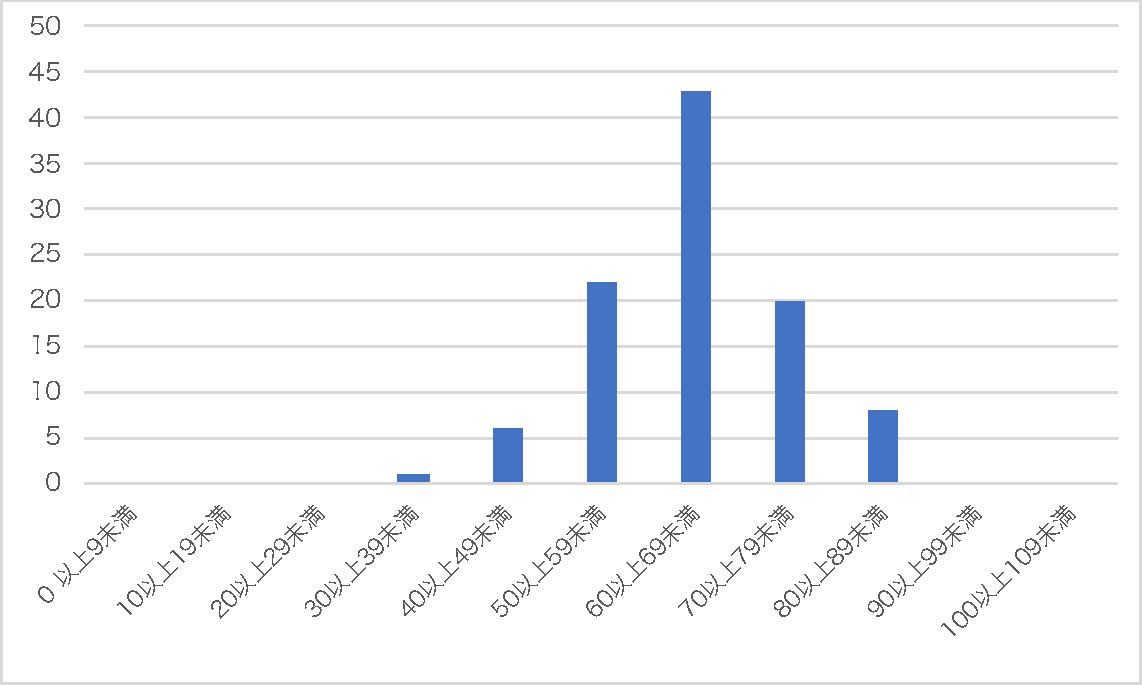
\includegraphics[width=10cm]{hist.pdf}
  \caption{ヒストグラム}
  \label{fig:histogram}
\end{figure}

\clearpage

\section{Excel実験}

\subsection{総和,平均,中央値,分散}

エクセルでの総和の計算は次の手順で行います.

\begin{enumerate}
    \item 総和を表示したいセルを選択する.
    \item ``=sum(''と入力する.
    \item 総和を計算したいセルを選択する.\footnote{データを選択する方法はいくつかあります.皆さんの慣れた方法でやってください.また,Excelも自動でいろいろやってくれるので,閉じカッコが保管される場合もあります.臨機応変に対応してください.}そうすると``(''の後ろにセル番号が入力される(図\ref{fig:sum}).
    \item )を入力する.
\end{enumerate}

\begin{figure}[htbp]
  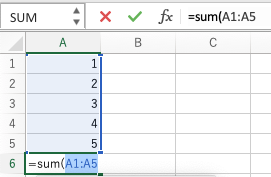
\includegraphics[width=10cm]{sum.png}
  \caption{総和を計算したいセルを選択した状態.}
  \label{fig:sum}
\end{figure}

同じやり方で,平均,分散,標準偏差が計算できます.平均なら``SUM''の部分を``MEAN''に変えます.代表値とexcelの関数の関係を表\ref{tab:funcs}に示します\footnote{分散や標準偏差に関連する関数は複数あります.それぞれ意味が違います.その意味はこの講義で扱う範疇を超えているので説明しません.興味がある人は調べてみましょう.}.

\begin{table}[htb]
    \centering
    \caption{代表値とExcelの関数}
    \begin{tabular}{|c|c|}
      \hline
      総和 & SUM\\ \hline
      平均 & MEAN\\ \hline
      分散 & VAR.P\\ \hline
      標準偏差 & STDEV.P \\ \hline
      最大値 & MAX \\ \hline
      最小値 & MIN \\ \hline
    \end{tabular}
    \label{tab:funcs}
\end{table}

\paragraph{演習}
csvの平均,分散,標準偏差を求めなさい.

\paragraph{演習}
csvの平均,中央値を求めなさい.そして,平均値と中央値の差について考察しなさい.

\subsection{度数分布表}
\label{sec:hist}

データから表のような度数分布表を作るにはどうすればよいでしょうか.
まず階級を設定します.
値が0から100の範囲であるとして,それを10刻みに分けるとします.
つまり,0から9,10から19,20から29,30から39,40から49,50から59,60から69,70から79,80から89,90から99,100
``FREQUENCY''

\footnote{``COUNTIFS''という関数を使っても度数分布表を作ることが可能です.}

\paragraph{演習}
csvデータから度数分布表を書け.

\subsection{ヒストグラム}

\ref{sec:hist}節で作成した度数分布表からグラフを作ります.
グラフで用いる数値は階級と度数です.
その2つを選択しましょう.
次に,グラフのヒストグラムをクリックします.
そうすると,ヒストグラムが出来上がります.

\paragraph{演習}

\ref{sec:hist}節の演習で作成した度数分布表に基づきヒストグラムをかけ.


\subsection{レポート提出}

提出は電子データで送る.データ形式はpdfもしくはdocxとする.

\section{おまけ}

ファイル形式

確率分布

ガウス分布

不偏分散


\chapter{Excelによる統計処理2}

\section{目的}

エクセルにはデータを解析するための関数が多く用意されている.今回はその一部を用い,データ解析の初歩を学ぶ.

\section{原理}

\subsection{グラフ}

データの特徴を視覚的に把握するためにグラフを用います.
代表的なグラフの一つが前回取り扱ったヒストグラムです.
ヒストグラム以外にも様々なグラフが存在します.
今回は,折れ線グラフ,円グラフ,散布図を取り扱います.

\paragraph{棒グラフ}

棒グラフは大きさの比較に用いられます.時間変化を把握するのに用いてはいけません.

\paragraph{折れ線グラフ}

値の時間変化の把握に用いられます.
大きさを比べる目的で折れ線グラフを使わないようにしましょう.

\paragraph{円グラフ}

割合をは把握するために用いられます.
扇型の角度は全体に対する割合を表します.
円グラフは合計で100\%にならなければなりません.

例えば,表\ref{tab:hist}

\paragraph{散布図}

データの値同士の関係性を知りたいときがあります.
値の関係性を見るために用いられます.
例えば,身長と体重の関係です.


\subsection{相関係数}

散布図では,視覚的に値同士の関係性を見ることができます.
しかし,定量的にどの程度関係しているか知りたいときには相関係数を使います.
相関係数は次の式で計算されます.
\begin{equation}
    \label{eq:1}
    r = \frac{\frac{1}{N} \sum_{i=1}^N (x_i - \bar{x})(y_i - \bar{y})}{\sqrt{\frac{1}{N} \sum_{i=1}^N (x_i - \bar{x})^2} \sqrt{\frac{1}{N} \sum_{i=1}^N}(y_i - \bar{y})^2}
\end{equation}
相関係数は直線的な関係かどうかをみることができます.
しかし,U字型であったりS字型の関係であった場合は相関係数ではみることができません.

正の相関
負の相関

\subsection{散布図と回帰直線}

平均に戻る.回帰.


\section{実験}

\subsection{折れ線グラフ}

手順は前回のヒストグラムと同じです.

\paragraph{演習}
csvファイルから折れ線グラフを作りなさい.ただし,横軸は 縦軸は にしなさい.

\subsection{円グラフ}

\paragraph{演習}


\subsection{折れ線グラフ}

表に示すデータを折れ線グラフにします.
横軸を,縦軸をとします.
よく軸のデータと縦軸のデータを選びます.
グラフの散布図の折れ線グラフを選びます.

\paragraph{演習}
csvファイルから折れ線グラフを作りなさい.ただし,横軸は 縦軸は にしなさい.


\subsection{散布図}

\paragraph{演習}

csvファイルから散布図をかきなさい.ただし,横軸は 縦軸は にしなさい.


\subsection{相関係数}

Excelで相関係数を求めるのは簡単です.前回の総和を求めたのと同じ要領で行います.しかし,今回は2列データがありますので,そこだけ注意しましょう.

CORREL

\paragraph{演習}
csvデータから相関係数を求めなさい.

\subsection{回帰直線}



\paragraph{演習}

csvデータから散布図と回帰直線を書きなさい.

\subsection{レポート提出}

提出は電子データで送る.データ形式はpdfもしくはdocxとする.


\section{おまけ}
R,python

プロット
R,matplotlib,gnuplot


有料ならmatlabがある.



\end{document}
